\documentclass[letter,12pt]{article}
\usepackage[top=2.0cm, bottom=2.0cm, left=2.0cm, right=2.0cm]{geometry}

% Configuración de Fira Sans para TODO el documento
\usepackage[sfdefault]{FiraSans} % Fuente principal
\usepackage{FiraMono}

\usepackage[utf8]{inputenc}
% Se configura diccionario en español y en entorno de tablas aparecerá el nombre Tabla x
\usepackage[spanish,es-tabla]{babel}
% Se utilizará el punto decimal en lugar de coma para definir números con decimales
\spanishdecimal{.}

% Tablas, imágenes y formato
\usepackage{graphicx}
\usepackage{array}
\usepackage{booktabs}
\usepackage{longtable}
\usepackage{tabularx}
\usepackage{multirow}
\usepackage{multicol}
\usepackage{makecell}
\usepackage{float}
\usepackage{enumitem}
\usepackage{setspace}
\usepackage{fancyhdr}

% Matemáticas y elementos gráficos
\usepackage{amsmath,mathtools,amsfonts,amssymb}
\usepackage{xcolor}
\usepackage{tikz}
\usepackage{tcolorbox}
\usepackage{pdfpages}

% Código y enlaces
\usepackage{listings}
\usepackage{hyperref}
\usepackage{xurl}

\setlength{\parindent}{0pt}
\setlength{\parskip}{0.55em}
\setlength{\headheight}{22pt}
\setlength{\emergencystretch}{2em}
\graphicspath{{./}}

% Colores institucionales UNAM
\definecolor{unamblue}{RGB}{0,51,102}
\definecolor{unamgold}{RGB}{153,126,48}
\definecolor{myred}{HTML}{911010}
\definecolor{myblue}{HTML}{142966}
\definecolor{myaqua}{HTML}{1EA69A}
\definecolor{backcolour}{rgb}{0.95,0.95,0.92}

\hypersetup{
	colorlinks=false,
	pdfborder={0 0 0},
	pdftitle={Proyecto final - Cempasúchil},
	pdfauthor={Equipo 8}
}

% Estilos de código
\lstdefinestyle{bashstyle}{
	backgroundcolor=\color{backcolour},
	basicstyle=\ttfamily\small,
	numbers=left,
	numberstyle=\tiny\color{gray},
	frame=single,
	tabsize=4,
	breaklines=true,
	captionpos=b,
	keywordstyle=\color{myblue},
	commentstyle=\color{myaqua},
	stringstyle=\color{myred},
	showstringspaces=false,
	columns=fullflexible,
	morekeywords={sudo,apt,git,cmake,open,cd,ls,mkdir,cp}
}
\lstdefinestyle{terminal}{
	backgroundcolor=\color{backcolour},
	basicstyle=\ttfamily\small,
	frame=single,
	tabsize=4,
	breaklines=true,
	showstringspaces=false,
	columns=fullflexible
}

% Recuadro provisional para las capturas
\newcommand{\capturapendiente}[2]{%
	\begin{figure}[H]
		\centering
		\fbox{%
			\parbox[c][5.2cm][c]{0.88\textwidth}{%
				\centering
				\textbf{Captura pendiente}\\[0.3cm]
				\textit{#1}%
			}%
		}
		\caption{#2}
	\end{figure}
}

%% Encabezado y pie de página %%
\pagestyle{fancy}  
\fancyhf{} 
\renewcommand{\headrule}{\hbox to\headwidth{\color{black}\leaders\hrule height \headrulewidth\hfill}}
\renewcommand{\headrulewidth}{0.4pt}
\fancyhead[L]{\color{black}\small{Computación Gráfica e Interacción Humano-Computadora}}
\fancyhead[R]{\color{black}\small{Proyecto final}}
\fancyfoot[R]{\small\thepage}

\onehalfspacing
\begin{document}
	\begin{titlepage}
		\thispagestyle{empty}
		\begin{center}
			\vspace{0.8cm}
			\begin{minipage}{0.125\textwidth}
				\centering
				
\includegraphics[width=\textwidth]{UNAM}
			\end{minipage}
			\hfill
			\begin{minipage}{0.7\textwidth}
				\centering
				{\color{black}\fontsize{16}{18}\selectfont
					\textbf{UNIVERSIDAD NACIONAL AUTÓNOMA DE MÉXICO} \\
					\vspace{0.3cm}
					\textbf{FACULTAD DE INGENIERÍA} \\
					\vspace{0.3cm}
					\textbf{COMPUTACIÓN GRÁFICA E INTERACCIÓN HUMANO-COMPUTADORA} \\
					\vspace{0.3cm}
					\textbf{SEMESTRE 2027 - 1}
				}
			\end{minipage}
			\hfill
			\begin{minipage}{0.125\textwidth}
				\centering
				
\includegraphics[width=\textwidth]{UNAM_INGENIERIA}
			\end{minipage}
			
			\vspace{1cm}
			
			\begin{tikzpicture}
				\draw[black, line width=1.5pt] (2\textwidth,0) -- (\textwidth,0);
			\end{tikzpicture}
			
			\vspace{1cm}
			
			{\color{black}\fontsize{18}{20}\selectfont
				\textbf{CEMPASÚCHIL: OFRENDA, MEMORIA Y TRADICIÓN} \\[0.3cm]
				{\fontsize{14}{16}\selectfont PROYECTO FINAL} \\
				\vspace{1.5cm}
			}
			
			{\color{black}\fontsize{14}{16}\selectfont
				\begin{tabular}{l r l}
					\textbf{ALUMNOS} & \textit{Basilio Illescas Andrés} & \textit{Product Owner} \\[0.3cm]
					& \textit{Trejo Olvera Emmanuel} & \textit{Scrum Master} \\[0.3cm]
					& \textit{Pérez Olvera Alexis Abraham} & \textit{Developer} \\[0.3cm]
					& \textit{Cruz Macedo Samuel Santiago} & \textit{Developer} \\[0.3cm]
					\textbf{PROFESOR} & \textit{Ing. José Ramón Pérez Athié} & \\[0.3cm]
					\textbf{GRUPO} & \textit{04} & \\[0.3cm]
				\end{tabular}
			}
			
			\vfill
			
			{\color{black}\fontsize{12}{14}\selectfont
				Ciudad Universitaria, CDMX \hfill Fecha de entrega: \today
			}
		\end{center}
	\end{titlepage}
	
	\newpage
	\thispagestyle{empty}
	\begin{center}
		{\fontsize{16}{20}\selectfont\textbf{HOJA DE EVIDENCIAS}}\\[0.8cm]
		{\fontsize{14}{18}\selectfont\textbf{Cempasúchil: ofrenda, memoria y tradición}}\\[0.3cm]
		{\large Proyecto final de Computación Gráfica e Interacción Humano-Computadora}\\[1.2cm]
		\renewcommand{\arraystretch}{2.0}
		\begin{tabular}{p{8.5cm}p{5.5cm}}
			\toprule
			\textbf{Alumno} & \textbf{Número de cuenta}\\
			\midrule
			Basilio Illescas Andrés & \rule{4.5cm}{0.4pt}\\
			Cruz Macedo Samuel Santiago & \rule{4.5cm}{0.4pt}\\
			Pérez Olvera Alexis Abraham & \rule{4.5cm}{0.4pt}\\
			Trejo Olvera Emmanuel & \rule{4.5cm}{0.4pt}\\
			\bottomrule
		\end{tabular}
	\end{center}

	\newpage
	\tableofcontents
	\newpage

	\section*{Resumen}
	\addcontentsline{toc}{section}{Resumen}
	Cempasúchil es una aplicación gráfica interactiva escrita en C++17 con OpenGL 3.3 y GLSL que recrea una noche de Día de Muertos. El visitante recorre un panteón, sigue un sendero de pétalos entre faroles, veladoras y papel picado, y llega a una ofrenda de tres niveles en el portal de una casa de adobe. El sistema reúne el pipeline gráfico completo visto en el curso: modelado jerárquico en Blender, intercambio en glTF 2.0, texturizado con mapas de color, rugosidad y normales, iluminación con un modelo de Phong y luces puntuales, transmisión con aproximación de Fresnel para vidrio y agua, un \textit{skybox} y nueve animaciones activables con el teclado. Tres animaciones se programaron directamente en OpenGL, tres se crearon en Blender y se reproducen a partir de pistas exportadas, y tres usan personajes con esqueleto cuyos clips se evalúan con \textit{skinning} lineal. El resultado cumple los requisitos mínimos de la especificación y se compila en macOS, Windows y Linux.

	\section{Introducción}
	El Día de Muertos es una de las celebraciones más representativas de México. La UNESCO inscribió en 2008 la festividad indígena dedicada a los muertos en la Lista Representativa del Patrimonio Cultural Inmaterial de la Humanidad (UNESCO, 2008). Sus elementos visuales (la flor de cempasúchil, el papel picado, las veladoras, la ofrenda escalonada y el camino de pétalos que guía a las almas) se prestan para un proyecto de graficación porque combinan geometría repetitiva, materiales translúcidos, fuentes de luz pequeñas y movimiento.

	La especificación del curso pide un sistema interactivo que recorra todas las etapas del pipeline gráfico: conceptualización, modelado geométrico, color, texturizado, iluminación, sombreado, animación, interacción y renderizado con OpenGL 3 o superior (Segal y Akeley, 2010). Para el sombreado se emplea el modelo de reflexión de Phong (1975), que separa las componentes ambiental, difusa y especular, y la aproximación de Schlick (1994) al término de Fresnel para que vidrios y líquidos reflejen más en ángulos rasantes. Los modelos se intercambian en glTF 2.0 (Khronos Group, 2021), un formato que conserva jerarquías de nodos, materiales PBR, esqueletos y clips de animación.

	En animación se usan tres familias de técnicas descritas en la literatura de tiempo real (Akenine-Möller et al., 2018; Gregory, 2018): transformaciones básicas aplicadas a una jerarquía, interpolación de \textit{keyframes} y animación procedural. Las trayectorias se interpolan con \textit{splines} de Catmull-Rom (Catmull y Rom, 1974), en su variante centrípeta para evitar lazos (Yuksel et al., 2011), y las rotaciones con interpolación esférica de cuaterniones (Shoemake, 1985). Los personajes con esqueleto se deforman con \textit{skinning} lineal por vértice, la técnica introducida por Magnenat-Thalmann et al. (1988) y que hoy es el estándar de glTF.

	Este reporte describe la metodología, los experimentos de validación y los resultados de la versión final. Las entregas parciales de prototipo, modelado, y texturizado, color e iluminación se integraron sin cambios de arquitectura; la última etapa añadió las animaciones y su interacción.

	\section{Objetivos}
	\subsection{Objetivo general}
	Desarrollar un sistema gráfico interactivo en OpenGL 3.3 que represente una ofrenda de Día de Muertos y aplique el pipeline gráfico completo, desde el modelado hasta la animación interactiva.

	\subsection{Objetivos específicos}
	\begin{itemize}[leftmargin=*]
		\item Integrar al menos ocho modelos propios y ocho modelos de librería, texturizados y organizados en un grafo de escena jerárquico.
		\item Iluminar la escena con al menos dos técnicas (Phong para materiales opacos y Fresnel para materiales translúcidos) y un mapa de entorno.
		\item Ofrecer al menos dos interacciones con luces en tiempo real.
		\item Integrar tres animaciones por código, tres creadas en software externo y dos animaciones por huesos, todas activables con el teclado.
		\item Mantener la compilación con CMake en macOS, Windows y Linux.
	\end{itemize}

	\section{Metodología práctica}

	\subsection{Metodología basada en prototipos}
	El trabajo siguió las fases de la metodología basada en prototipos de la especificación. En la recolección de requisitos se eligió el tema, se definieron las interacciones y se acotó el alcance de cada entrega. El diseño conceptual produjo la distribución de la escena (panteón al norte, sendero al centro y casa con ofrenda al sur) y el catálogo de modelos. A partir de ahí se construyó un primer prototipo con geometría gris, que en cada entrega se probó, se corrigió y se amplió: primero con modelado completo, después con texturas e iluminación, y al final con animación. La Tabla~\ref{tab:fases} resume cómo se recorrió cada fase.

	\begin{table}[H]
		\centering
		\small
		\begin{tabularx}{\textwidth}{p{4.2cm}X}
			\toprule
			\textbf{Fase} & \textbf{Actividad en el proyecto}\\
			\midrule
			Requisitos y planificación & Tema ``México y su cultura'' con la ofrenda de Día de Muertos; lista de modelos, luces e interacciones mínimas. \\
			Diseño conceptual & Plano de la escena, eje del sendero como \textit{spline} y flujo de navegación en primera persona. \\
			Prototipo inicial & Ventana GLFW, carga glTF, cámara y grafo de escena con geometría sin textura. \\
			Validación y retroalimentación & Revisión del equipo en cada entrega parcial; ajustes de escala, intersecciones y rendimiento. \\
			Iteración y mejoras & Texturas PBR, luces puntuales, filtrado de luces, \textit{skybox} y animaciones. \\
			Implementación completa & Integración de las nueve animaciones con entrada por teclado y documentación. \\
			\bottomrule
		\end{tabularx}
		\caption{Fases de la metodología basada en prototipos.}
		\label{tab:fases}
	\end{table}

	\subsection{Organización del equipo}
	Dentro de cada fase se trabajó con iteraciones cortas al estilo \textit{Scrum}. La Tabla~\ref{tab:roles} muestra los roles.

	\begin{table}[H]
		\centering
		\small
		\begin{tabularx}{\textwidth}{p{5.2cm}p{3.0cm}X}
			\toprule
			\textbf{Integrante} & \textbf{Rol} & \textbf{Responsabilidad}\\
			\midrule
			Basilio Illescas Andrés & Product Owner & Priorizar elementos y revisar que la escena represente el tema. \\
			Trejo Olvera Emmanuel & Scrum Master & Coordinar avances, retirar bloqueos e integrar el sistema floral. \\
			Pérez Olvera Alexis Abraham & Developer & Modelar objetos de la ofrenda y verificar su integración. \\
			Cruz Macedo Samuel Santiago & Developer & Modelar elementos arquitectónicos y ambientales. \\
			\bottomrule
		\end{tabularx}
		\caption{Roles del equipo.}
		\label{tab:roles}
	\end{table}

	\subsection{Herramientas y tecnologías}
	\begin{table}[H]
		\centering
		\small
		\begin{tabularx}{\textwidth}{p{4.0cm}X}
			\toprule
			\textbf{Herramienta} & \textbf{Uso}\\
			\midrule
			C++17 & Aplicación, grafo de escena, interacción y animación. \\
			OpenGL 3.3 Core y GLSL 330 & Renderizado, materiales, iluminación y recorte por plano. \\
			Blender 5.2 (Blender Foundation, 2026) & Modelado, horneado de texturas, animación de papel, pétalos y jarra, y esqueletos de personajes. \\
			glTF 2.0 y cgltf & Intercambio de modelos, materiales, esqueletos y clips. \\
			GLFW, GLAD y GLM & Ventana y entrada, carga de funciones OpenGL y matemáticas. \\
			stb\_image & Lectura de PNG y JPEG en Windows y Linux. \\
			CMake & Configuración multiplataforma. \\
			\bottomrule
		\end{tabularx}
		\caption{Herramientas empleadas.}
		\label{tab:herramientas}
	\end{table}

	\subsection{Modelado y composición de la escena}
	Los modelos propios se construyeron en Blender a partir de primitivas con extrusión, superficies de revolución y modificadores, y se exportaron a glTF conservando su jerarquía. Así, el altar se descompone en sus tres niveles y el farol en poste, brazo y lámpara. La aplicación replica esa jerarquía como nodos editables: cada nodo guarda traslación, rotación y escala locales, y su matriz de mundo se obtiene como $M_{\text{mundo}} = M_{\text{padre}}\, T\, R\, S$.

	La escena final tiene 2\,132 nodos, 77 modelos distintos y 10\,548 instancias. Los elementos que se repiten miles de veces (pétalos, veladoras, flores y bardas) se agrupan en lotes y se dibujan con \texttt{glDrawElementsInstanced}, con una matriz y un tinte por instancia. El sendero es una \textit{spline} Catmull-Rom centrípeta, evaluada con el algoritmo de Barry y Goldman (1988) y reparametrizada por longitud de arco; con ella se colocan pétalos, veladoras, faroles y papel picado a distancias regulares. La Figura~\ref{fig:general} muestra la distribución.

	\begin{figure}[H]
		\centering
		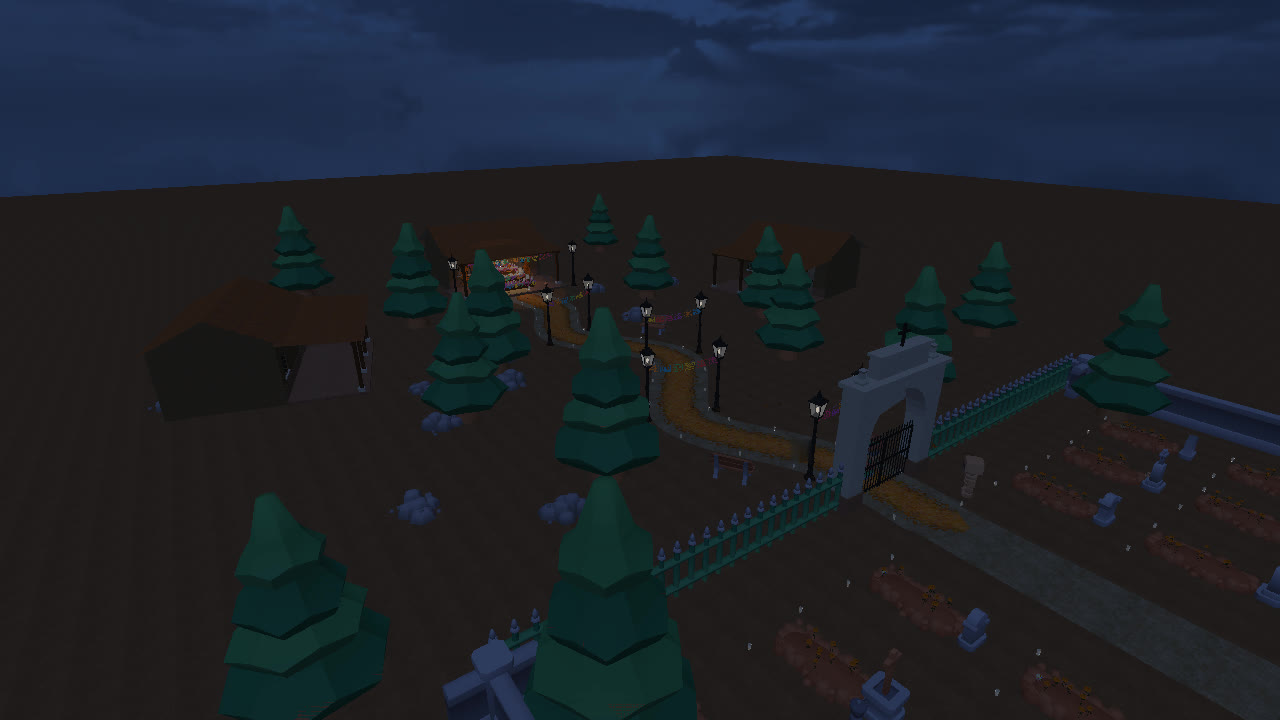
\includegraphics[width=0.85\textwidth]{images/vista-general.jpg}
		\caption{Vista general: panteón, sendero de pétalos y casa con la ofrenda.}
		\label{fig:general}
	\end{figure}

	\subsection{Texturizado, color e iluminación}
	Las texturas de los modelos propios se diseñaron con nodos procedurales en Blender y se hornearon a mapas de color, rugosidad y normales. En el \textit{fragment shader} las normales se perturban sin tangentes precalculadas: las derivadas \texttt{dFdx} y \texttt{dFdy} de la posición y de las coordenadas UV dan la base tangente de cada píxel. Los pétalos y el papel picado usan recorte alfa para mostrar su silueta sin geometría adicional.

	La iluminación combina dos técnicas:
	\begin{itemize}[leftmargin=*]
		\item \textbf{Phong} para materiales opacos: una luz direccional lunar azulada y hasta 25 luces puntuales (veladoras, cirios y faroles) con atenuación cuadrática. El brillo especular se deriva de la rugosidad del material.
		\item \textbf{Fresnel} para vidrio y agua: la aproximación de Schlick mezcla el color transmitido con un reflejo que crece en ángulos rasantes. Así se ven los vasos, las jarras y las veladoras.
	\end{itemize}
	El entorno es un \textit{skybox} con mapa cúbico. Su \textit{vertex shader} elimina la traslación de la vista para que el horizonte no se mueva, y su \textit{fragment shader} oscurece el atardecer original hacia un tono nocturno. Para no recorrer luces inútiles, el renderizador filtra por caja envolvente las luces que pueden alcanzar a cada objeto y descarta las primitivas fuera de cámara con los planos del \textit{frustum} extraídos de la matriz de vista y proyección (Gribb y Hartmann, 2001).

	\subsection{Animación}
	La especificación pide animaciones de tres tipos (básica, por \textit{keyframes} y procedural) y tres medios (código, software externo y huesos). La Tabla~\ref{tab:animaciones} relaciona cada animación con su tecla, su medio y su técnica. Todas se coordinan desde la clase \texttt{Animaciones} (\texttt{src/scene/Animaciones.cpp}). Esta clase recibe la tecla, avanza cada animación con el tiempo del cuadro y escribe el resultado en los nodos del grafo de escena o en los \textit{uniforms} del renderizador.

	\begin{table}[H]
		\centering
		\small
		\begin{tabularx}{\textwidth}{c p{3.3cm} p{2.4cm} X}
			\toprule
			\textbf{Tecla} & \textbf{Animación} & \textbf{Medio} & \textbf{Técnica}\\
			\midrule
			1 & Mariposa monarca & Código & Máquina de estados, \textit{keyframes} sobre Catmull-Rom y aleteo procedural en la jerarquía cuerpo-alas. \\
			2 & Recorrido de cámara & Código & Siete \textit{keyframes} de posición y mira con interpolación suave. \\
			3 & Veladoras & Código & Estados de encendido y apagado; encendido por grupos y parpadeo procedural en GLSL. \\
			4 & Papel picado & Blender & \textit{Shape keys} horneadas en una caché de vértices de 96 cuadros. \\
			5 & Remolino de pétalos & Blender & \textit{Keyframes} de 720 pétalos exportados como pistas. \\
			6 & Jarra sirviendo agua & Blender & \textit{Keyframes} de la jarra, nivel del agua y chorro exportados como pistas. \\
			7 & Visitante 1 & Huesos & \textit{Armature} de siete huesos; caminata, depósito de la ofrenda y reverencia. \\
			8 & Visitante 2 & Huesos & Segundo personaje; observa una tumba, saluda y baila. \\
			9 & Esqueleto bailando & Huesos & Baile de 12 s con cinco pasos mezclados. \\
			L & Faroles & Código & Interacción de luz: apagado y encendido gradual. \\
			\bottomrule
		\end{tabularx}
		\caption{Animaciones e interacciones disponibles.}
		\label{tab:animaciones}
	\end{table}

	\subsubsection{Animaciones por código}
	\textbf{Mariposa monarca (1).} Una mariposa reposa sobre el petate frente al altar. Al presionar la tecla, recorre la máquina de estados reposo, despegue, vuelo y aterrizaje. La ruta se define con diez puntos de control que pasan por el reposo, suben frente al arco y regresan; se interpola con la misma clase \texttt{Camino} del sendero y se recorre a velocidad constante. Los estados se distinguen por la distancia recorrida: en los primeros y últimos 0.6 m el aleteo crece o se apaga, y en el tramo central alcanza su amplitud completa. Las alas son nodos hijos del cuerpo, de modo que basta rotarlas alrededor de su bisagra para que acompañen la traslación y la orientación del cuerpo. Es un ejemplo de jerarquía de transformaciones.

	\textbf{Recorrido de cámara (2).} Siete \textit{keyframes} de posición y siete de punto de mira describen la entrada desde el panteón, el cruce de la portada, el sendero y la llegada a la ofrenda. Ambas secuencias se interpolan con Catmull-Rom y comparten un parámetro de tiempo suavizado con $3t^2 - 2t^3$, de modo que la cámara arranca y se detiene sin saltos. Mientras dura el recorrido se ignora la entrada de movimiento; la misma tecla lo interrumpe.

	\textbf{Veladoras (3).} Una máquina de estados en C++ pasa por encendidas, apagando, apagadas y encendiendo. Cada estado fija dos valores que llegan al \textit{shader}: un frente de encendido sobre el eje Z y un nivel global. En GLSL, la función \texttt{factorVela} agrupa las velas en tramos de 4.4 m. Cada tramo enciende cuando el frente lo alcanza, así que las velas se prenden por grupos desde el panteón hasta el altar. El mismo factor agrega un parpadeo procedural: dos senoidales con una fase pseudoaleatoria por vela. El factor modula tanto la emisión de las flamas como la luz puntual que cada vela proyecta sobre su entorno.

	\textbf{Faroles (L).} La segunda interacción de luz reduce gradualmente a cero la emisión y la luz de los faroles, y la restablece al presionar de nuevo.

	\subsubsection{Animaciones creadas en Blender}
	Las tres animaciones de software externo se modelaron y animaron en Blender. Para el motor se hornearon en datos que OpenGL reproduce sin depender de Blender.

	\textbf{Papel picado (4).} Seis pliegos se deforman con \textit{shape keys} (borde fijo, curvatura y onda) animadas por \textit{keyframes} con fases y amplitudes distintas. El resultado se horneó como caché de vértices de 96 cuadros; en cada cuadro el motor copia las posiciones al búfer de vértices. La tecla calma o reanuda el viento: la velocidad de reproducción baja o sube de forma gradual.

	\textbf{Remolino de pétalos (5).} En Blender, un \textit{script} calculó los \textit{keyframes} de posición y rotación de 720 pétalos: se levantan del sendero, giran en una espiral de dos brazos frente al altar y se asientan con vaivén. El \textit{script} \texttt{exportar\_remolino.py} lee la escena cuadro por cuadro y guarda, por pétalo, su posición, su cuaternión y su escala en el archivo binario \texttt{remolino\_petalos.pist}. Durante la conversión cambia los ejes de Blender ($Z$ arriba) a los de OpenGL ($Y$ arriba). En el motor los pétalos forman un lote instanciado. Cada cuadro se interpolan los dos cuadros vecinos de la pista y se reescriben las 720 matrices con \texttt{glBufferSubData}.

	\textbf{Jarra sirviendo agua (6).} La jarra gira alrededor de un pivote en su pico. El agua interior se recorta con una caja cuya altura está animada para que la superficie se mantenga horizontal y el volumen se conserve; el chorro es una curva con bisel animado; el vaso se llena con una \textit{shape key}. El \textit{script} \texttt{exportar\_jarra.py} exporta la posición y rotación de la jarra, la altura de la superficie, el llenado del vaso y los factores del chorro. En OpenGL el recorte del agua se resuelve con un plano: el \textit{fragment shader} descarta los fragmentos con $\mathbf{n}\cdot\mathbf{p} + d > 0$. El chorro es un tubo cuyos anillos se recolocan sobre la curva exportada en cada cuadro.

	\subsubsection{Animaciones por huesos}
	Los personajes parten de las piezas del \textit{Kenney Graveyard Kit} (Kenney, 2021), con licencia CC0. El \textit{script} \texttt{exportar\_personajes.py} crea en Blender un \textit{armature} de siete huesos (cadera, torso, cabeza, brazos y piernas), une las piezas en una malla y liga cada pieza a su hueso. Después genera los clips (reposo, caminar, caminar cargando, depositar, incorporarse, reverencia, observar, saludar, baile corto y baile completo) y exporta cada personaje como glTF con \textit{skin} y una animación por clip.

	En el motor, \texttt{Modelo::posar} interpola las pistas de traslación y rotación de cada hueso (lineal y esférica), calcula sus matrices globales y aplica \textit{skinning} lineal:
	\begin{equation}
		\mathbf{v}' = \sum_{i} w_i \, G_i \, B_i^{-1} \, \mathbf{v},
	\end{equation}
	donde $G_i$ es la matriz global del hueso, $B_i^{-1}$ su matriz inversa de \textit{bind} y $w_i$ el peso del vértice. Los vértices deformados se suben al búfer de la malla y la caja envolvente se recalcula para el descarte por \textit{frustum}. Entre clips hay una mezcla de 0.25 s para evitar saltos de pose.

	La trayectoria de cada personaje se describe en código como una secuencia de tramos (caminar por una ruta, girar, ejecutar un clip). Al caminar, la fase del ciclo avanza con la distancia recorrida (0.95 m por ciclo), lo que evita que los pies patinen. El visitante 1 lleva un pan de muerto colgado de un nodo ancla hijo del antebrazo; al terminar el clip de depósito, el pan queda sobre el primer piso del altar.

	\subsection{Interacción}
	La navegación es en primera persona, con caminata o vuelo libre. La Tabla~\ref{tab:controles} resume los controles.

	\begin{table}[H]
		\centering
		\small
		\begin{tabularx}{\textwidth}{p{3.8cm}X}
			\toprule
			\textbf{Entrada} & \textbf{Acción}\\
			\midrule
			W, A, S, D & Caminar por la escena. \\
			Shift & Aumentar la velocidad. \\
			Ratón y TAB & Orientar la cámara; TAB activa o libera el ratón. \\
			F, Q, E & Alternar vuelo libre; descender y ascender en vuelo. \\
			Rueda del ratón & Ajustar la velocidad de desplazamiento. \\
			1 a 9 & Iniciar las animaciones de la Tabla~\ref{tab:animaciones}. \\
			L & Apagar o encender los faroles. \\
			F2 & Alternar sólido y malla de alambre. \\
			R & Regresar a la entrada del panteón. \\
			Esc & Cerrar la aplicación. \\
			\bottomrule
		\end{tabularx}
		\caption{Controles de la aplicación.}
		\label{tab:controles}
	\end{table}

	\subsection{Fotografías de la ofrenda}
	Los siete portarretratos del altar están colocados, pero las fotografías quedan pendientes para la versión que presentará el equipo. Cada foto es la malla \texttt{foto} del modelo de portarretrato. Para cambiarla se edita su textura en \path{modelos-blender/portarretratos/portarretratos_texturizados.blend} y se vuelve a exportar el glTF; el procedimiento está en la sección ``Fotos de la ofrenda'' del \texttt{README.md}.

	\section{Experimentos}

	\subsection{Compilación en distintas plataformas}
	El proyecto se compiló con CMake en macOS (Xcode), Windows (Visual Studio 2022 y 2026) y Linux (GCC). Las pruebas de las entregas anteriores encontraron problemas que siguen resueltos en esta versión:
	\begin{itemize}[leftmargin=*]
		\item Fuera de macOS no aparecían las texturas porque la decodificación de imágenes solo existía con ImageIO; se integró \texttt{stb\_image} para Windows y Linux.
		\item En pantallas con escalado, el tamaño lógico de la ventana no coincide con el del \textit{framebuffer}, así que se usa \texttt{glfwGetFramebufferSize} antes de \texttt{glViewport}.
		\item \texttt{Rutas.cpp} localiza \texttt{assets/} y \texttt{shaders/} desde la ruta real del ejecutable, con rutas anchas en Windows, para no depender del directorio de trabajo.
		\item Las diferencias de redondeo entre compiladores cambian en unas pocas piezas el conteo de la ofrenda; una diferencia pequeña se registra como aviso.
		\item El controlador VirtIO de una máquina virtual con Windows 11 ARM no expuso OpenGL 3.3, por lo que la aplicación requiere un controlador con OpenGL 3.3 real.
	\end{itemize}

	\subsection{Validación de las animaciones}
	Las animaciones se probaron en Linux sobre Mesa (\texttt{llvmpipe}, OpenGL 4.5 Core) dentro de un servidor X virtual. Un \textit{script} externo al repositorio abría la aplicación en una vista fija, enviaba las teclas con \texttt{xdotool} y tomaba capturas a intervalos con FFmpeg. Así se comprobó cada animación sin intervención manual. Las capturas de la sección de resultados provienen de esas corridas. Se verificó además:
	\begin{itemize}[leftmargin=*]
		\item que las pistas exportadas tuvieran el tamaño esperado: 264 cuadros $\times$ 720 pétalos $\times$ 8 valores para el remolino, y 240 cuadros $\times$ 13 valores para la jarra;
		\item que la jarra arrancara a 18 cm del vaso, se inclinara 60° durante el vertido y que el vaso pasara de 3~\% a 82~\% de llenado;
		\item que cada personaje tuviera siete articulaciones y todos sus clips, con la duración en cuadros definida en Blender;
		\item que el pan del visitante 1 quedara apoyado en el hueco frontal del primer piso, sin intersecar las calaveritas ni los cirios.
	\end{itemize}

	\subsection{Rendimiento}
	Como el motor ya filtraba luces por caja envolvente y descartaba por \textit{frustum}, las animaciones nuevas se diseñaron para no alterar esos mecanismos. El remolino actualiza un solo búfer de instancias por cuadro. Los personajes deforman en CPU mallas de pocos cientos de vértices. La jarra solo recalcula el tubo del chorro mientras está visible. Ninguna animación agrega llamadas de dibujo por elemento animado.

	\section{Resultados}

	\subsection{Cumplimiento de requisitos}
	La Tabla~\ref{tab:requisitos} contrasta los requisitos mínimos de la especificación con lo implementado.

	\begin{table}[H]
		\centering
		\small
		\begin{tabularx}{\textwidth}{p{6.2cm}X}
			\toprule
			\textbf{Requisito} & \textbf{Implementación}\\
			\midrule
			8 modelos de librería o modelados & 25 modelos de Kenney Graveyard Kit (tumbas, criptas, rejas, cipreses, personajes). \\
			8 modelos creados por participantes & Más de 40 modelos propios: altar, arco, flor, pétalo, veladoras, cirios, pan, calaverita, papel picado, portarretratos, jarra, vaso, farol, casa, portada, platos y dulces. \\
			2 interacciones con luces & Veladoras (3) y faroles (L). \\
			\textit{Skybox} y texturas en modelos propios & Mapa cúbico nocturno y texturas horneadas en todos los modelos propios. \\
			2 animaciones de huesos & Visitante 1 (7), visitante 2 (8) y esqueleto bailando (9). \\
			3 animaciones por código & Mariposa (1), recorrido de cámara (2) y veladoras (3). \\
			3 animaciones de software externo & Papel picado (4), remolino de pétalos (5) y jarra (6). \\
			8 animaciones con input & Nueve teclas (1 a 9) más L. \\
			Phong y Fresnel & Phong en materiales opacos; Fresnel de Schlick en vidrio y agua. \\
			\bottomrule
		\end{tabularx}
		\caption{Requisitos mínimos y su cumplimiento.}
		\label{tab:requisitos}
	\end{table}

	\subsection{Capturas de la aplicación}
	Las Figuras~\ref{fig:panteon} a \ref{fig:ofrenda} muestran las zonas principales de la escena, y las Figuras~\ref{fig:anim1} a \ref{fig:faroles} cada animación en curso.

	\begin{figure}[H]
		\centering
		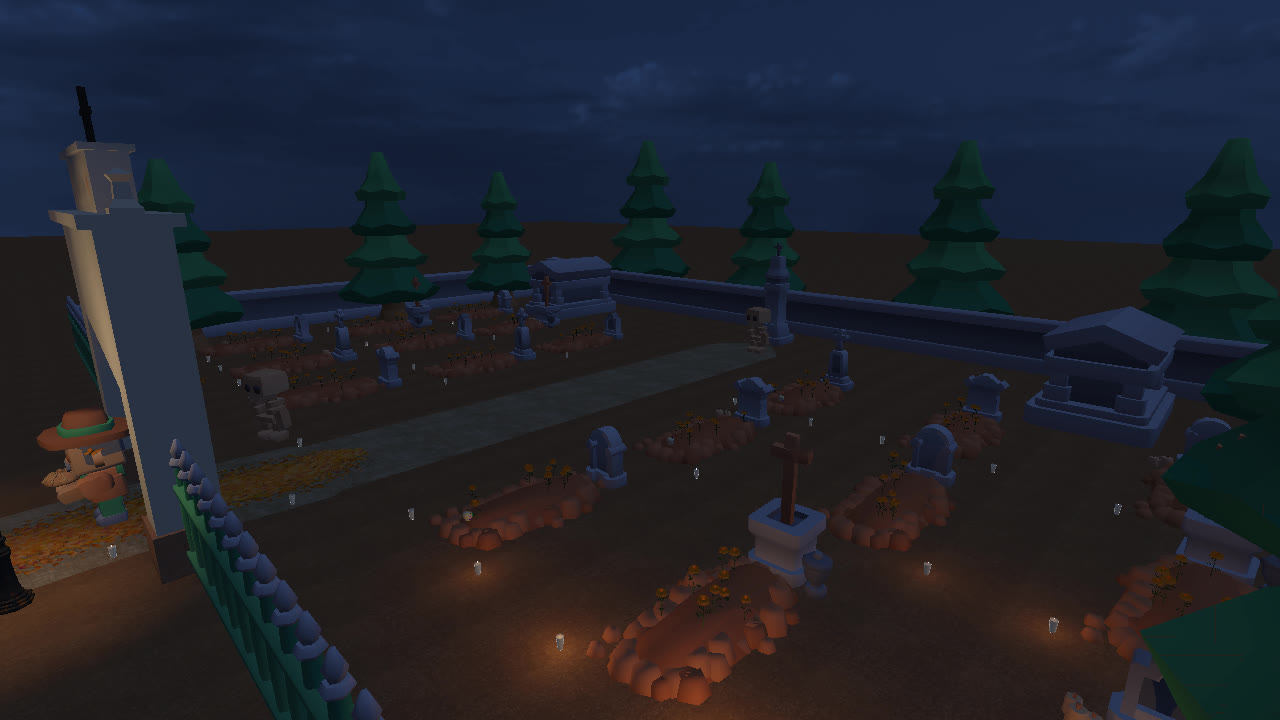
\includegraphics[width=0.85\textwidth]{images/panteon.jpg}
		\caption{Panteón con tumbas, criptas y cipreses de la librería.}
		\label{fig:panteon}
	\end{figure}

	\begin{figure}[H]
		\centering
		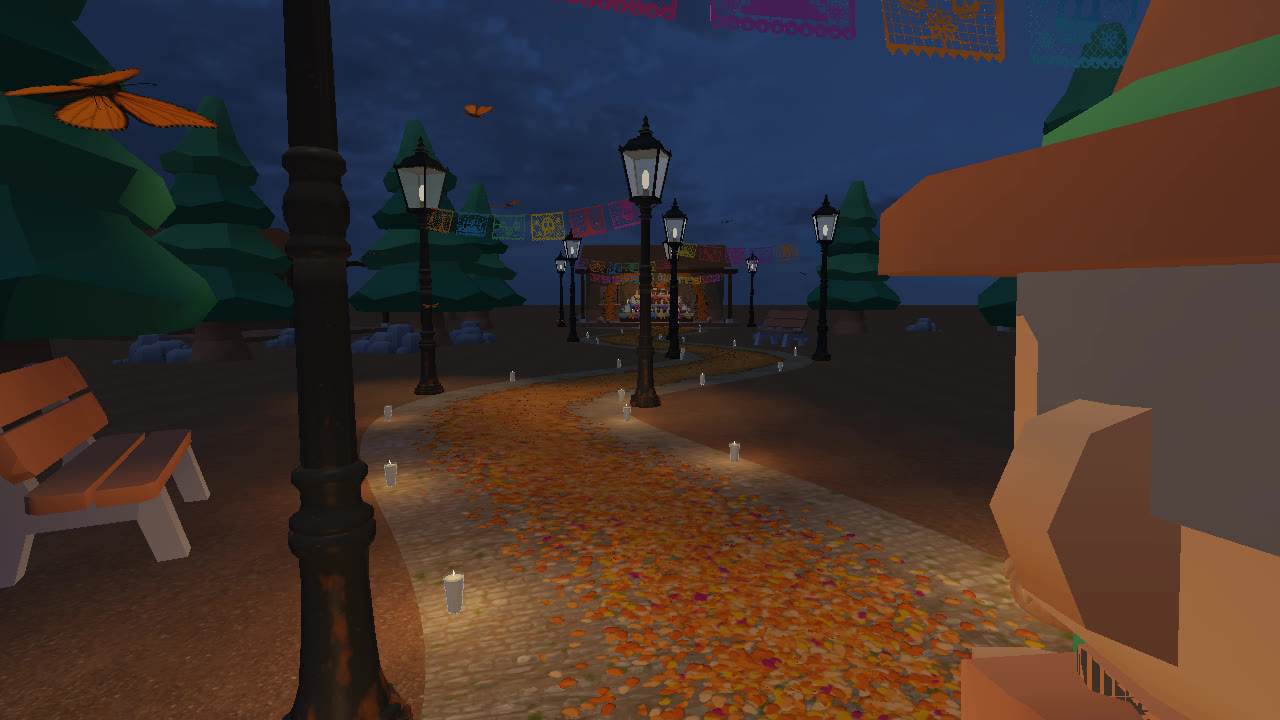
\includegraphics[width=0.85\textwidth]{images/camino.jpg}
		\caption{Sendero de pétalos con veladoras, faroles y papel picado.}
		\label{fig:camino}
	\end{figure}

	\begin{figure}[H]
		\centering
		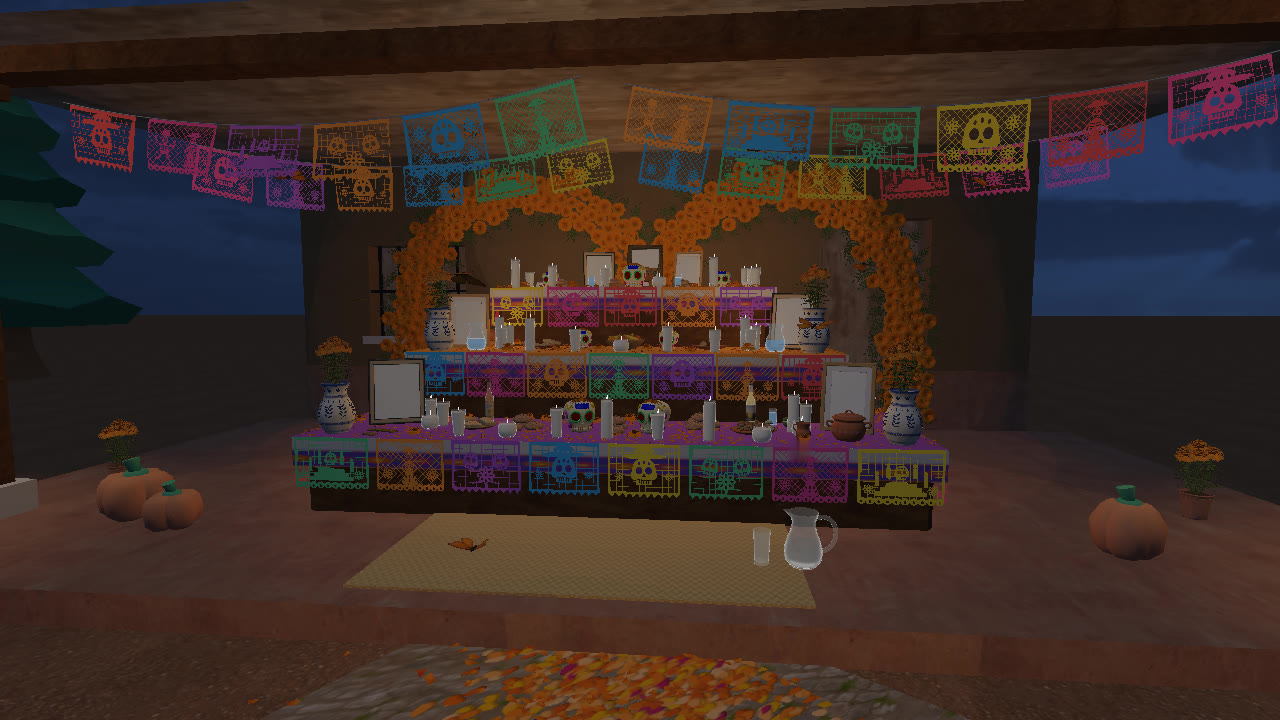
\includegraphics[width=0.85\textwidth]{images/ofrenda.jpg}
		\caption{Ofrenda de tres niveles en el portal de la casa de adobe.}
		\label{fig:ofrenda}
	\end{figure}

	\begin{figure}[H]
		\centering
		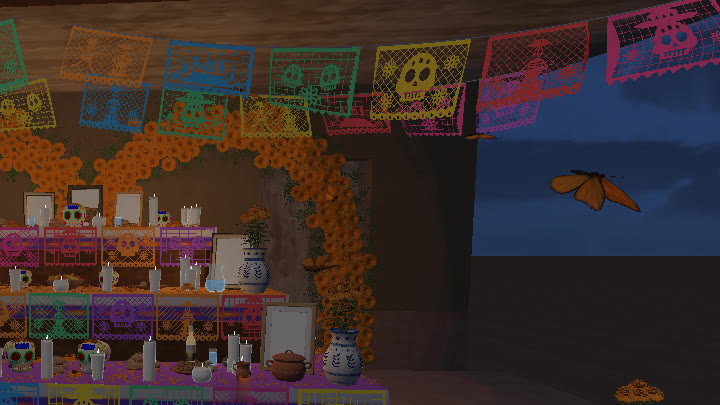
\includegraphics[width=0.85\textwidth]{images/anim-1-mariposa.jpg}
		\caption{Animación 1: la mariposa monarca en pleno vuelo frente al altar.}
		\label{fig:anim1}
	\end{figure}

	\begin{figure}[H]
		\centering
		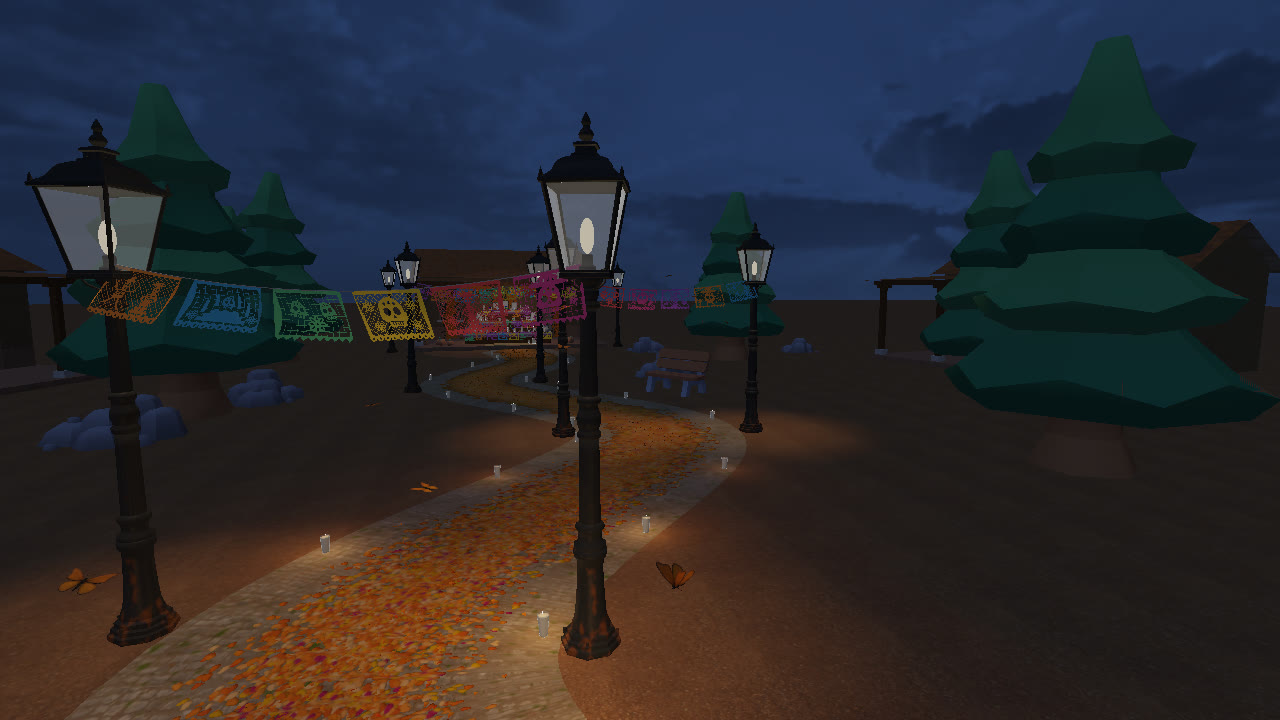
\includegraphics[width=0.85\textwidth]{images/anim-2-recorrido.jpg}
		\caption{Animación 2: cuadro intermedio del recorrido de cámara por el sendero.}
		\label{fig:anim2}
	\end{figure}

	\begin{figure}[H]
		\centering
		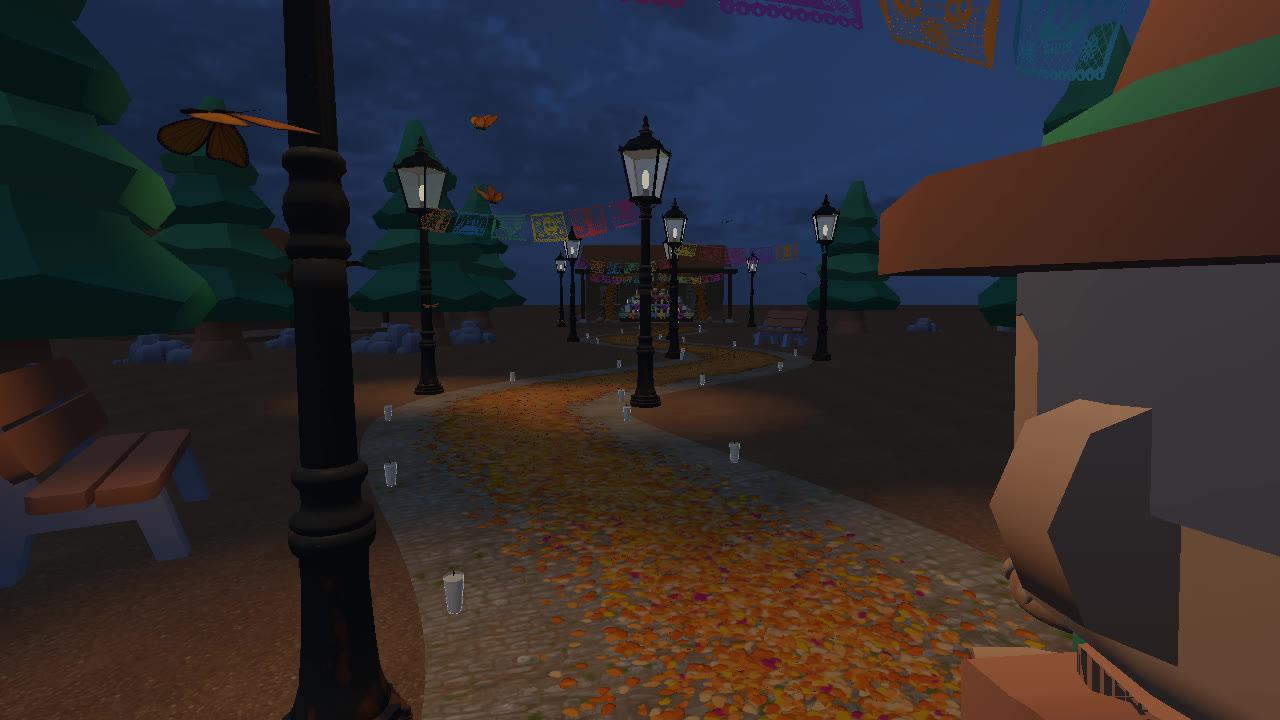
\includegraphics[width=0.49\textwidth]{images/anim-3-veladoras-a.jpg}\hfill
		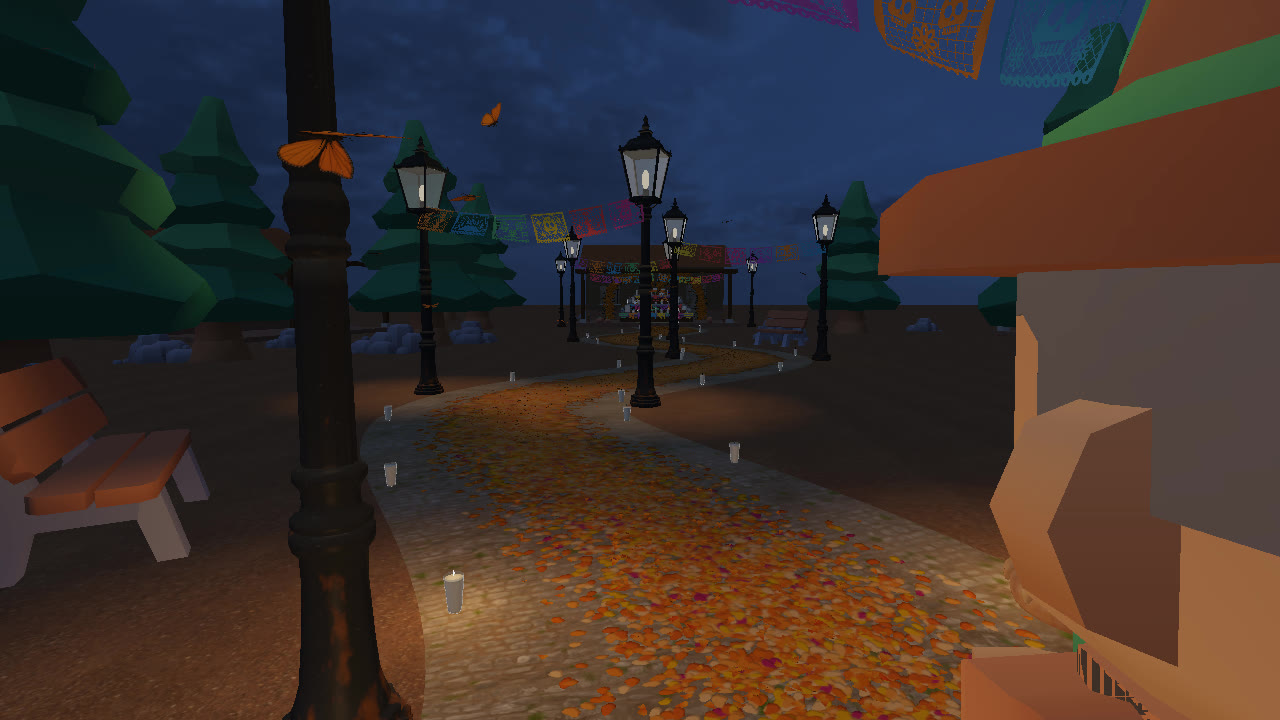
\includegraphics[width=0.49\textwidth]{images/anim-3-veladoras-b.jpg}
		\caption{Animación 3: veladoras apagadas (izquierda) y encendiéndose por grupos (derecha).}
		\label{fig:anim3}
	\end{figure}

	\begin{figure}[H]
		\centering
		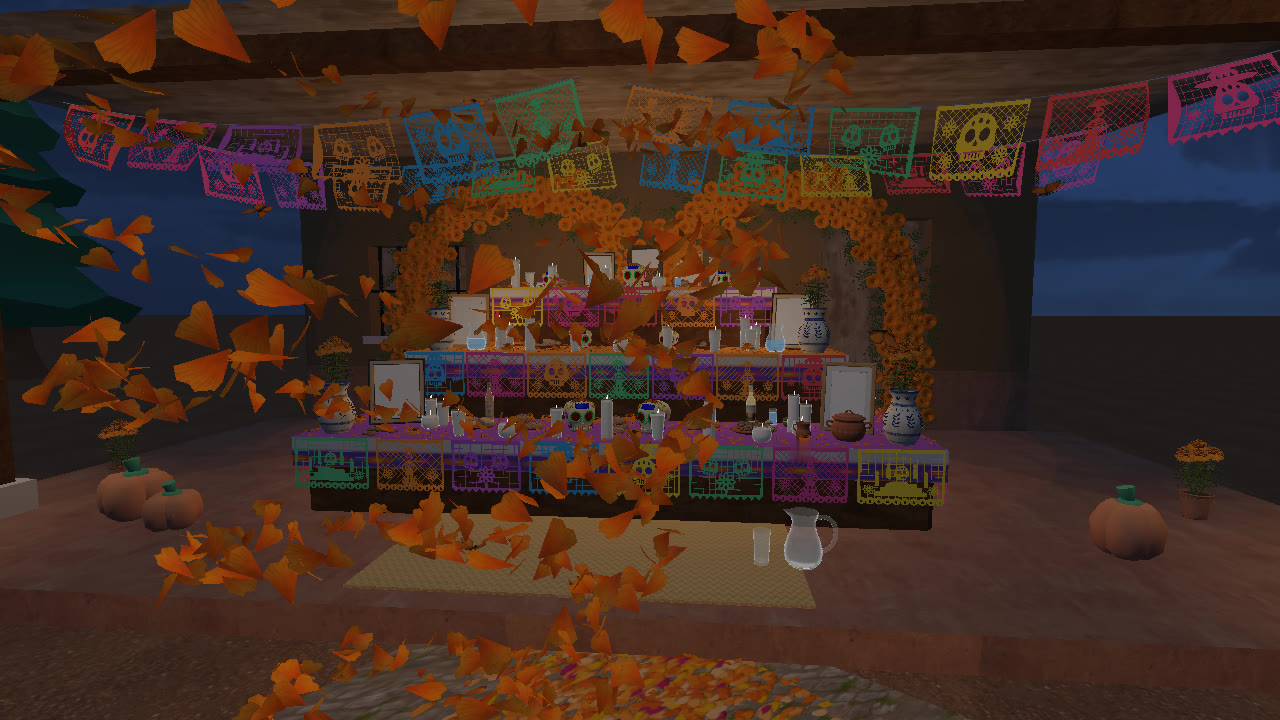
\includegraphics[width=0.85\textwidth]{images/anim-5-remolino.jpg}
		\caption{Animación 5: los pétalos forman la espiral frente a la ofrenda.}
		\label{fig:anim5}
	\end{figure}

	\begin{figure}[H]
		\centering
		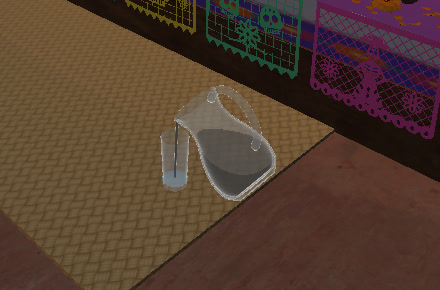
\includegraphics[width=0.6\textwidth]{images/anim-6-jarra.jpg}
		\caption{Animación 6: la jarra vierte agua en el vaso sobre el petate.}
		\label{fig:anim6}
	\end{figure}

	\begin{figure}[H]
		\centering
		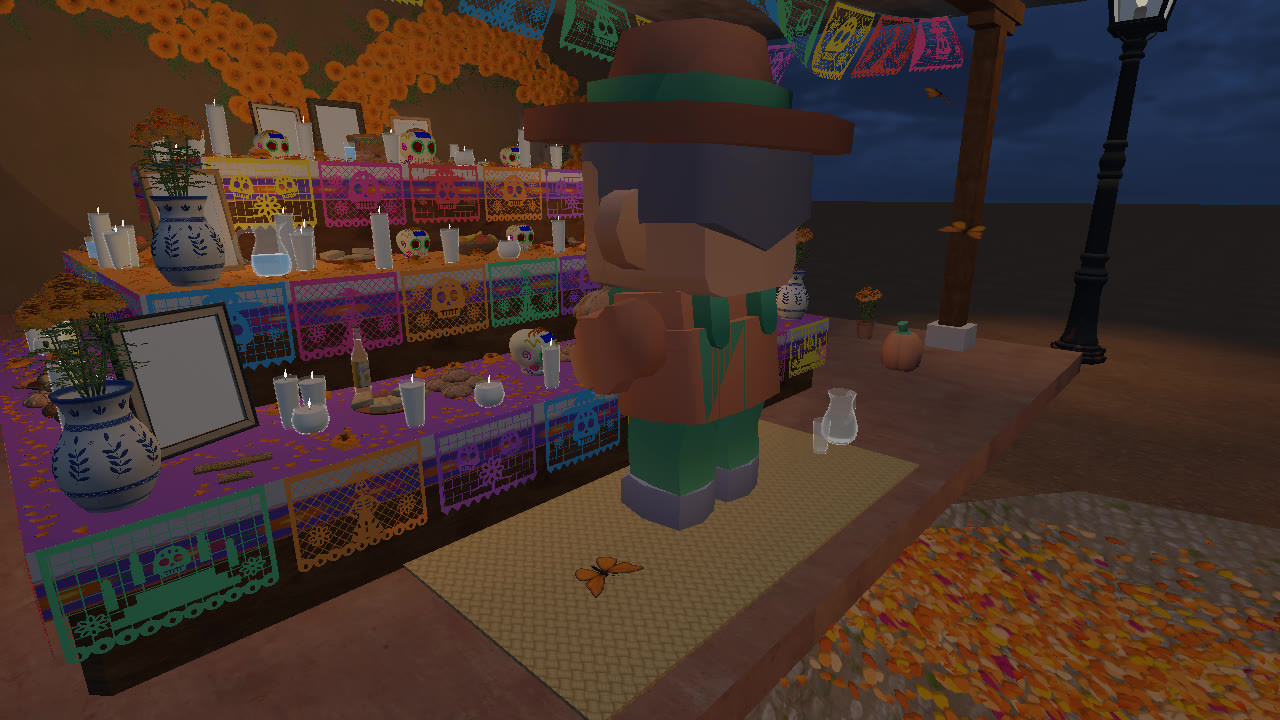
\includegraphics[width=0.85\textwidth]{images/anim-7-visitante.jpg}
		\caption{Animación 7: el visitante deja el pan de muerto en el primer piso del altar.}
		\label{fig:anim7}
	\end{figure}

	\begin{figure}[H]
		\centering
		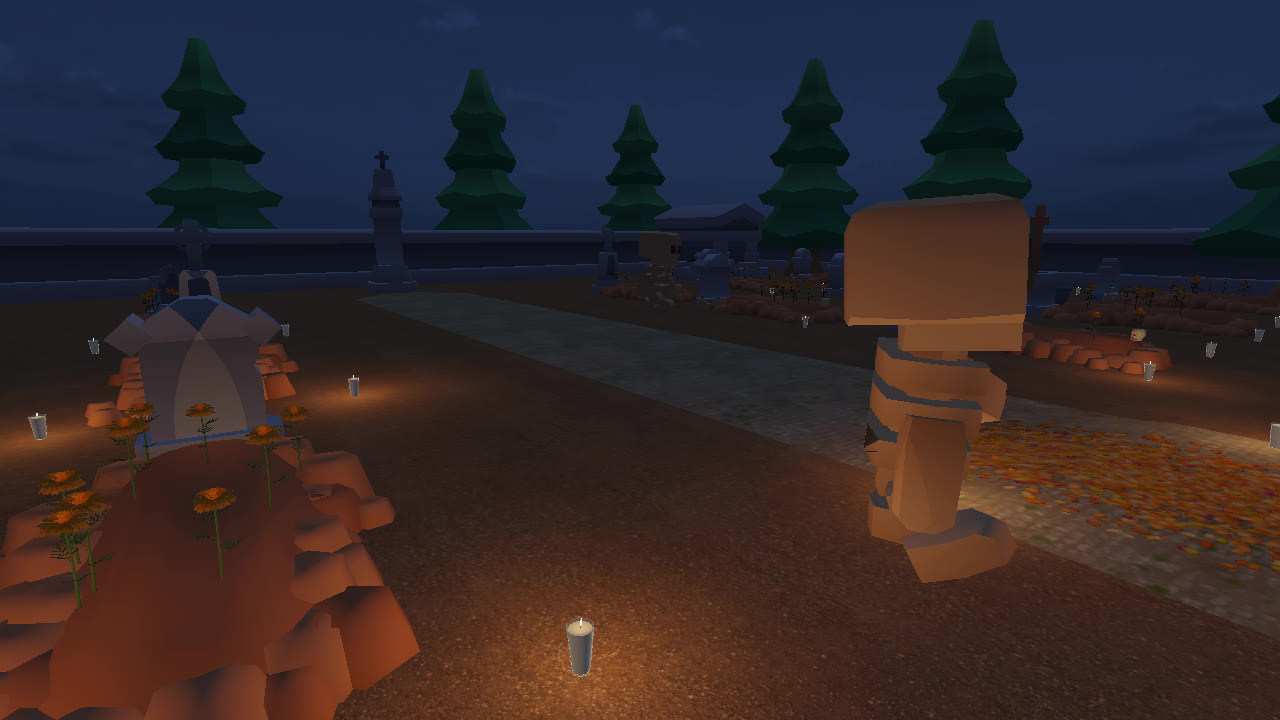
\includegraphics[width=0.85\textwidth]{images/anim-8-9-panteon.jpg}
		\caption{Animaciones 8 y 9: el visitante 2 recorre el panteón mientras el esqueleto baila junto a la portada.}
		\label{fig:anim8}
	\end{figure}

	\begin{figure}[H]
		\centering
		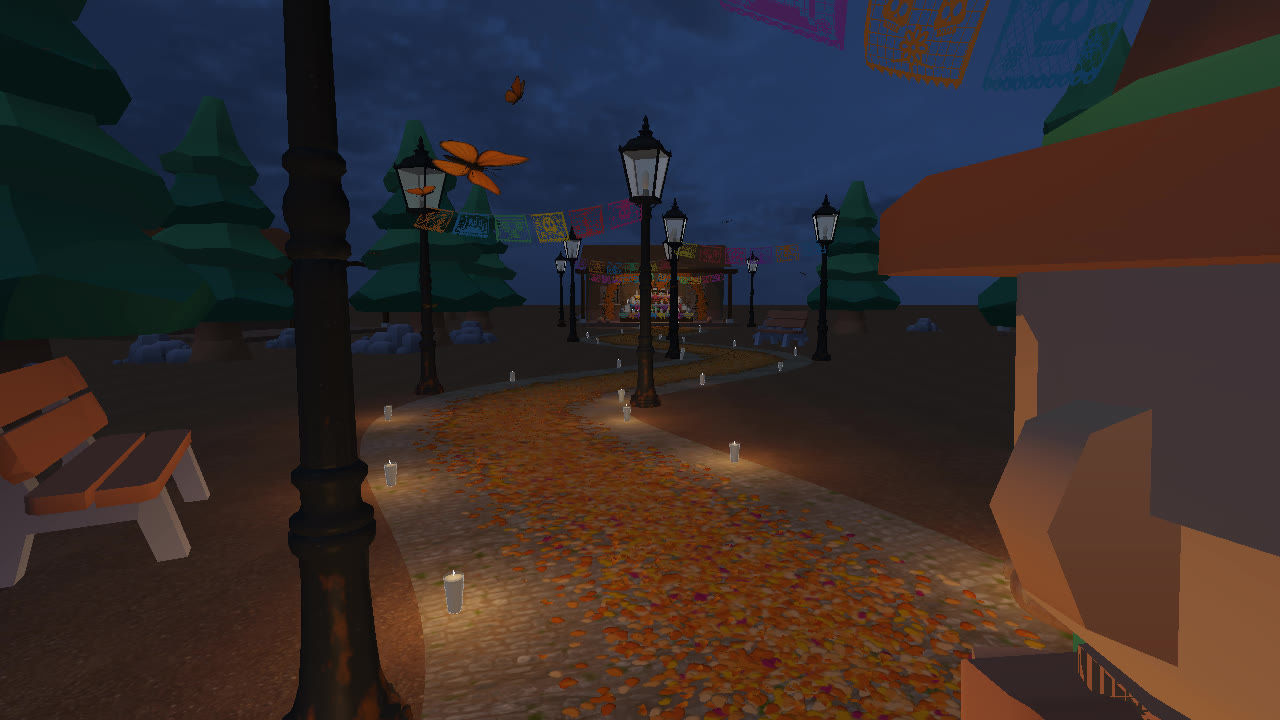
\includegraphics[width=0.85\textwidth]{images/faroles-apagados.jpg}
		\caption{Interacción L: sendero con los faroles apagados; solo quedan las veladoras.}
		\label{fig:faroles}
	\end{figure}

	\section{Conclusiones individuales}

	\subsection*{Basilio Illescas Andrés}
	\textit{Pendiente de redactar por el integrante.}

	\subsection*{Cruz Macedo Samuel Santiago}
	\textit{Pendiente de redactar por el integrante.}

	\subsection*{Pérez Olvera Alexis Abraham}
	\textit{Pendiente de redactar por el integrante.}

	\subsection*{Trejo Olvera Emmanuel}
	\textit{Pendiente de redactar por el integrante.}

	\section{Video demostrativo}
	Enlace al video de 3 a 5 minutos: \textit{(por agregar)}.

	\section{Referencias}
	\begin{itemize}[leftmargin=*]
		\item Akenine-Möller, T., Haines, E., Hoffman, N., Pesce, A., Iwanicki, M. y Hillaire, S. (2018). \textit{Real-time rendering} (4.ª ed.). CRC Press.
		\item Barry, P. J. y Goldman, R. N. (1988). A recursive evaluation algorithm for a class of Catmull-Rom splines. \textit{ACM SIGGRAPH Computer Graphics, 22}(4), 199--204. \url{https://doi.org/10.1145/378456.378511}
		\item Blender Foundation. (2026). \textit{Blender 5.2 manual}. \url{https://docs.blender.org/manual/es/latest/}
		\item Catmull, E. y Rom, R. (1974). A class of local interpolating splines. En R. E. Barnhill y R. F. Riesenfeld (Eds.), \textit{Computer aided geometric design} (pp. 317--326). Academic Press.
		\item Gregory, J. (2018). \textit{Game engine architecture} (3.ª ed.). CRC Press.
		\item Gribb, G. y Hartmann, K. (2001). \textit{Fast extraction of viewing frustum planes from the world-view-projection matrix}. \url{https://www.gamedevs.org/uploads/fast-extraction-viewing-frustum-planes-from-world-view-projection-matrix.pdf}
		\item Kenney. (2021). \textit{Graveyard kit} [Modelos 3D, licencia CC0]. \url{https://kenney.nl/assets/graveyard-kit}
		\item Khronos Group. (2021). \textit{glTF 2.0 specification}. \url{https://registry.khronos.org/glTF/specs/2.0/glTF-2.0.html}
		\item Magnenat-Thalmann, N., Laperrière, R. y Thalmann, D. (1988). Joint-dependent local deformations for hand animation and object grasping. En \textit{Proceedings of Graphics Interface '88} (pp. 26--33). Canadian Information Processing Society.
		\item Phong, B. T. (1975). Illumination for computer generated pictures. \textit{Communications of the ACM, 18}(6), 311--317. \url{https://doi.org/10.1145/360825.360839}
		\item Schlick, C. (1994). An inexpensive BRDF model for physically-based rendering. \textit{Computer Graphics Forum, 13}(3), 233--246. \url{https://doi.org/10.1111/1467-8659.1330233}
		\item Segal, M. y Akeley, K. (2010). \textit{The OpenGL graphics system: A specification (version 3.3, core profile)}. Khronos Group. \url{https://registry.khronos.org/OpenGL/specs/gl/glspec33.core.pdf}
		\item Shoemake, K. (1985). Animating rotation with quaternion curves. \textit{ACM SIGGRAPH Computer Graphics, 19}(3), 245--254. \url{https://doi.org/10.1145/325165.325242}
		\item UNESCO. (2008). \textit{La festividad indígena dedicada a los muertos}. Patrimonio Cultural Inmaterial. \url{https://ich.unesco.org/es/RL/la-festividad-indigena-dedicada-a-los-muertos-00054}
		\item Yuksel, C., Schaefer, S. y Keyser, J. (2011). Parameterization and applications of Catmull-Rom curves. \textit{Computer-Aided Design, 43}(7), 747--755. \url{https://doi.org/10.1016/j.cad.2010.08.008}
	\end{itemize}
\end{document}
